\documentclass{ximera}


\newcommand{\RR}{\mathbb R}
\renewcommand{\d}{\,d}
\newcommand{\dd}[2][]{\frac{d #1}{d #2}}
\renewcommand{\l}{\ell}
\newcommand{\ddx}{\frac{d}{dx}}
\newcommand{\dfn}{\textbf}
\newcommand{\eval}[1]{\bigg[ #1 \bigg]}


\title[Dig-In:]{The derivative via limits} %% I don't know about this title

\begin{document}
\begin{abstract}
We compute the instantaneous growth rate by computing the limit of
average growth rates.
\end{abstract}
\maketitle


Given a function, it is often useful to know the rate at which the
function changes. To give you a feeling why this is true, consider the
following:
\begin{itemize}
\item If $s(t)$ represents the displacement (position relative to an
  origin) of an object with respect to time, the rate of change gives
  the velocity of the object.
\item If $v(t)$ represents the velocity of an object with respect to
  time, the rate of change gives the acceleration of the object.
\item If $R(x)$ represents the revenue generated by selling $x$
  objects, the rate of change gives us the \textit{marginal revenue},
  meaning the additional revenue generated by selling one additional
  unit. Note, there is an implicit assumption that $x$ is quite large
  compared to $1$.
\item If $C(x)$ represents the cost to produce $x$ objects, the rate
  of change gives us the \textit{marginal cost}, meaning the
  additional cost generated by selling one additional unit. Again,
  there is an implicit assumption that $x$ is quite large compared to
  $1$.
\item If $P(x)$ represents the profit gained by selling $x$ objects,
  the rate of change gives us the \textit{marginal profit}, meaning
  the additional cost generated by selling one additional unit. Again,
  there is an implicit assumption that $x$ is quite large compared to
  $1$.
\item The rate of change of a function can help us approximate a
  complicated function with a simple function.
\item The rate of change of a function can be used to help us solve
  equations that we would not be able to solve via other methods.
\end{itemize}

\begin{xarmaBoost}
What other examples can you find where one is interested in a ``rate
of change?''
\begin{freeResponse}
Answers will vary.
\end{freeResponse}
\end{xarmaBoost}

\section{From average velocity to instantaneous velocity}

%%
%% I'm still not totally happy with this section
%%

Perhaps the most concrete example of a ``rate of change'' that we are
interested in is the first example above:
\begin{quote}
  If $s(t)$ represents the displacement (position relative to an origin)
  of an object with respect to time, the rate of change gives the
  velocity of the object.
\end{quote}
When one computes average velocity, we look at 
\[
\frac{\text{change in displacement}}{\text{change in time}}.
\]
To obtain the (instantaneous) velocity, we want the change in time to
``go to'' zero. By this point we should know that ``go to'' is a
buzz-word for a \textit{limit}. The change in time is often given as
an interval, by something like
\[
I = [a, a+h].
\]
However, intervals must always be written 
\[
[a,b]
\]
where $a < b$. Given $I = [a, a+h]$, we see that $h$ cannot be
negative, or else it violates the notation for intervals. Hence, if we
want smaller, and smaller, intervals around a point $a$, and we want
$h$ to be able to be negative, we write
\[
I_h = 
\begin{cases}
  [a+h,a]  & \text{if $h<0$}, \\ %% note this is MORE correct than std books
  [a,a+h]  & \text{if $0<h$}.     %% in the content section, we can explain this in detail
\end{cases}
\]
Regardless of the value of $h$, the average velocity is computed by
\[
\frac{\text{change in displacement}}{\text{change in time}} =
\frac{s(t+h)-s(t)}{h}.
\]

Let's put this together by working an example.

\begin{example}
The \textit{MOOCulus Team} recently took a road trip from Columbus
Ohio to Urbana-Champaign Illinois in the \textit{MOOCulus-Mobile}. The
position of the MOOCulus-Mobile is roughly modeled by
\[
s(t) = 36t^2 - 4.8t^3 \qquad\text{(miles West of Columbus)} %% note the model is wrong
\]
on the interval $[0,5]$, where $t$ is measured in hours. The average
velocity on the interval $[0,5]$ is \answer[given]{60} miles per hour. On the
other hand, consider the interval
\[
I_h = 
\begin{cases}
  [1+h,1]  & \text{if $h<0$}, \\ %% note this is MORE correct than std books
  [1,1+h]  & \text{if $0<h$}.     %% in the content section, we can explain this in detail
\end{cases}
\]
When $h = 0.1$, the average velocity is \answer[given]{59.712}. On the other
hand, when $h=-0.1$, the average velocity is \answer[given]{55.392}.
\end{example}

Now let's change gears a bit. Displacement and velocity are good
metaphors for concepts in calculus. However, another powerful
metaphor comes from geometry, and this metaphor is too important to
postpone any longer.


\section{From slopes of secant lines to slopes of tangent lines}

You've been computing average rates of change for a while now, the
computation is simply
\[
\frac{\text{change in the function}}{\text{change in the input to the
    function}}.
\]
However, the question remains: Given a function that represents an
amount, how exactly does one find the function that will give the
instantaneous rate of change? Recall that the instantaneous rate of change
of a line is the slope of the line.  Hence the instantaneous rate of
change of a function is the slope of the tangent line. For now,
consider the following informal definition of a \textit{tangent line}:
\begin{quote}\index{tangent line}
Given a function $f(x)$, if one can ``zoom in''
on $f(x)$ sufficiently so that $f(x)$ seems to be a straight line,
then that line is the \dfn{tangent line} to $f(x)$ at the point
determined by $x$.
\end{quote}
We illustrate this informal definition with the following diagram:
\begin{image}
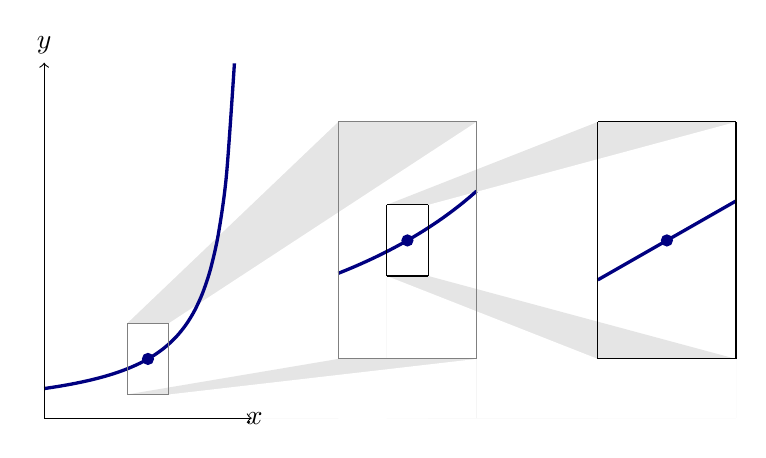
\begin{tikzpicture}
  \colorlet{penColor}{blue!50!black}
  \colorlet{penColor2}{red!50!black}
  \colorlet{textColor}{black}
  \colorlet{background}{white}
	\begin{axis}[
            domain=0:6, range=0:7,
            ymin=-.2,ymax=7,
            width=\textwidth,
            height=7cm, %% Hard coded height! Moreover this effects the aspect ratio of the zoom--sort of BAD
            axis lines=none,
          ]   
          \addplot [draw=none, fill=textColor!10!background] plot coordinates {(.8,1.6) (2.834,5)} \closedcycle; %% zoom fill
          \addplot [draw=none, fill=textColor!10!background] plot coordinates {(2.834,5) (4.166,5)} \closedcycle; %% zoom fill
          \addplot [draw=none, fill=background] plot coordinates {(1.2,1.6) (4.166,5)} \closedcycle; %% zoom fill
          \addplot [draw=none, fill=background] plot coordinates {(.8,1.6) (1.2,1.6)} \closedcycle; %% zoom fill

          \addplot [draw=none, fill=textColor!10!background] plot coordinates {(3.3,3.6) (5.334,5)} \closedcycle; %% zoom fill
          \addplot [draw=none, fill=textColor!10!background] plot coordinates {(5.334,5) (6.666,5)} \closedcycle; %% zoom fill
          \addplot [draw=none, fill=background] plot coordinates {(3.7,3.6) (6.666,5)} \closedcycle; %% zoom fill
          \addplot [draw=none, fill=background] plot coordinates {(3.3,3.6) (3.7,3.6)} \closedcycle; %% zoom fill
          
          \addplot [draw=none, fill=textColor!10!background] plot coordinates {(3.7,2.4) (6.666,1)} \closedcycle; %% zoom fill
          \addplot [draw=none, fill=textColor!10!background] plot coordinates {(3.3,2.4) (3.7,2.4)} \closedcycle; %% zoom fill
          \addplot [draw=none, fill=background] plot coordinates {(3.3,2.4) (5.334,1)} \closedcycle; %% zoom fill          
          \addplot [draw=none, fill=background] plot coordinates {(5.334,1) (6.666,1)} \closedcycle; %% zoom fill
          

          \addplot [draw=none, fill=textColor!10!background] plot coordinates {(.8,.4) (2.834,1)} \closedcycle; %% zoom fill
          \addplot [draw=none, fill=textColor!10!background] plot coordinates {(2.834,1) (4.166,1)} \closedcycle; %% zoom fill
          \addplot [draw=none, fill=background] plot coordinates {(1.2,.4) (4.166,1)} \closedcycle; %% zoom fill
          \addplot [draw=none, fill=background] plot coordinates {(.8,.4) (1.2,.4)} \closedcycle; %% zoom fill

          \addplot[very thick,penColor, smooth,domain=(0:1.833)] {-1/(x-2)};
          \addplot[very thick,penColor, smooth,domain=(2.834:4.166)] {3.333/(2.050-.3*x)-0.333}; %% 2.5 to 4.333
          %\addplot[very thick,penColor, smooth,domain=(5.334:6.666)] {11.11/(1.540-.09*x)-8.109}; %% 5 to 6.833
          \addplot[very thick,penColor, smooth,domain=(5.334:6.666)] {x-3}; %% 5 to 6.833
          
          \addplot[color=penColor,fill=penColor,only marks,mark=*] coordinates{(1,1)};  %% point to be zoomed
          \addplot[color=penColor,fill=penColor,only marks,mark=*] coordinates{(3.5,3)};  %% zoomed pt 1
          \addplot[color=penColor,fill=penColor,only marks,mark=*] coordinates{(6,3)};  %% zoomed pt 2

          \addplot [->,textColor] plot coordinates {(0,0) (0,6)}; %% axis
          \addplot [->,textColor] plot coordinates {(0,0) (2,0)}; %% axis
          
          \addplot [textColor!50!background] plot coordinates {(.8,.4) (.8,1.6)}; %% box around pt
          \addplot [textColor!50!background] plot coordinates {(1.2,.4) (1.2,1.6)}; %% box around pt
          \addplot [textColor!50!background] plot coordinates {(.8,1.6) (1.2,1.6)}; %% box around pt
          \addplot [textColor!50!background] plot coordinates {(.8,.4) (1.2,.4)}; %% box around pt
          
          \addplot [textColor!50!background] plot coordinates {(2.834,1) (2.834,5)}; %% zoomed box 1
          \addplot [textColor!50!background] plot coordinates {(4.166,1) (4.166,5)}; %% zoomed box 1
          \addplot [textColor!50!background] plot coordinates {(2.834,1) (4.166,1)}; %% zoomed box 1
          \addplot [textColor!50!background] plot coordinates {(2.834,5) (4.166,5)}; %% zoomed box 1

          \addplot [textColor] plot coordinates {(3.3,2.4) (3.3,3.6)}; %% box around zoomed pt
          \addplot [textColor] plot coordinates {(3.7,2.4) (3.7,3.6)}; %% box around zoomed pt
          \addplot [textColor] plot coordinates {(3.3,3.6) (3.7,3.6)}; %% box around zoomed pt
          \addplot [textColor] plot coordinates {(3.3,2.4) (3.7,2.4)}; %% box around zoomed pt

          \addplot [textColor] plot coordinates {(5.334,1) (5.334,5)}; %% zoomed box 2
          \addplot [textColor] plot coordinates {(6.666,1) (6.666,5)}; %% zoomed box 2
          \addplot [textColor] plot coordinates {(5.334,1) (6.666,1)}; %% zoomed box 2
          \addplot [textColor] plot coordinates {(5.334,5) (6.666,5)}; %% zoomed box 2

          \node at (axis cs:2.2,0) [anchor=east] {$x$};
          \node at (axis cs:0,6.6) [anchor=north] {$y$};
        \end{axis}
\end{tikzpicture}
%% \caption{Given a function $f(x)$, if one can ``zoom in''
%% on $f(x)$ sufficiently so that $f(x)$ seems to be a straight line,
%% then that line is the \textbf{tangent line} to $f(x)$ at the point
%% determined by $x$.}
%% \label{figure:informal-tangent}
\end{image}



The \textit{derivative} of a function $f(x)$ at $x$, is the instantaneous
rate of change, and hence is the slope of the tangent line at $x$. To
find the slope of this line, we consider \textit{secant} lines, lines
that locally intersect the curve at two points.  The slope of any
secant line that passes through the points $(x,f(x))$ and $(x+h,
f(x+h))$ is given by
\[
\frac{\Delta y}{\Delta x}=\frac{f(x+h) -f(x)}{(x+h)-x} =
\frac{f(x+h)-f(x)}{h}.
\]
%see Figure~\ref{figure:limit-dfn}. 
This leads to the \textit{limit definition of the derivative}:

%\begin{definitionOfTheDerivative}\index{limit!definition of the derivative}\index{derivative!limit definition}
\begin{definition}
The \dfn{derivative} of $f(x)$ is the function
\[
\ddx f(x) = \lim_{h\to 0} \frac{f(x+h) - f(x)}{h}.
\]
If this limit does not exist for a given value of $x$, then $f(x)$ is
not \dfn{differentiable} at $x$.
\end{definition}
%\end{definitionOfTheDerivative}
%\begin{marginfigure}[-1.75in]
\begin{image}
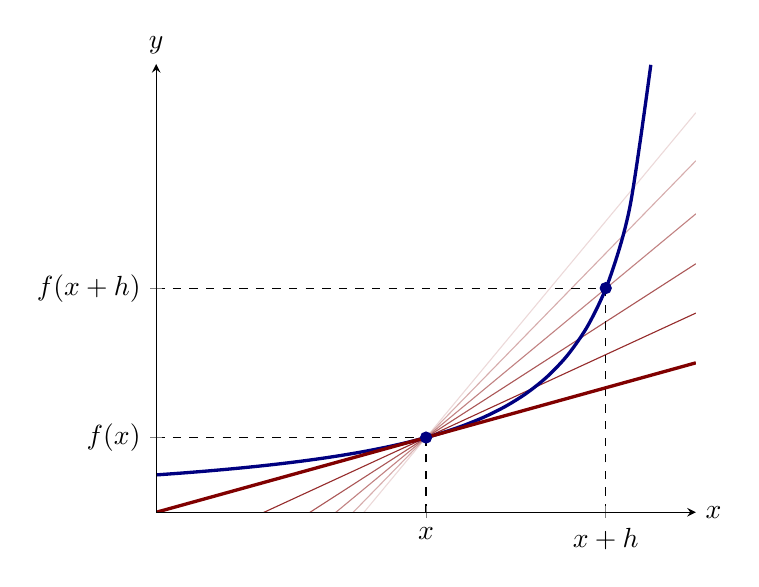
\begin{tikzpicture}
  \colorlet{penColor}{blue!50!black}
  \colorlet{penColor2}{red!50!black}
  \colorlet{textColor}{black}
  \colorlet{background}{white}  
	\begin{axis}[
            domain=0:2, range=0:6,ymax=6,ymin=0,
            axis lines =left, xlabel=$x$, ylabel=$y$,
            every axis y label/.style={at=(current axis.above origin),anchor=south},
            every axis x label/.style={at=(current axis.right of origin),anchor=west},
            xtick={1,1.666}, ytick={1,3},
            xticklabels={$x$,$x+h$}, yticklabels={$f(x)$,$f(x+h)$},
            axis on top,
          ]         
          \addplot [penColor2!15!background, domain=(0:2)] {-3.348+4.348*x};
          \addplot [penColor2!32!background, domain=(0:2)] {-2.704+3.704*x};
          \addplot [penColor2!49!background, domain=(0:2)] {-1.994+2.994*x};         
          \addplot [penColor2!66!background, domain=(0:2)] {-1.326+2.326*x}; 
          \addplot [penColor2!83!background, domain=(0:2)] {-0.666+1.666*x};
	  \addplot [textColor,dashed] plot coordinates {(1,0) (1,1)};
          \addplot [textColor,dashed] plot coordinates {(0,1) (1,1)};
          \addplot [textColor,dashed] plot coordinates {(0,3) (1.666,3)};
          \addplot [textColor,dashed] plot coordinates {(1.666,0) (1.666,3)};
          \addplot [very thick,penColor, smooth,domain=(0:1.833)] {-1/(x-2)};
          \addplot[color=penColor,fill=penColor,only marks,mark=*] coordinates{(1.666,3)};  %% closed hole          
          \addplot[color=penColor,fill=penColor,only marks,mark=*] coordinates{(1,1)};  %% closed hole          
          \addplot [very thick,penColor2, smooth,domain=(0:2)] {x};
        \end{axis}
\end{tikzpicture}
\end{image}
%% \caption{Tangent lines can be found as the limit of secant lines. The slope of the tangent line is given by
%% $\lim_{h\to 0} \frac{f(x+h) - f(x)}{h}.$}
%%  \label{figure:limit-dfn}
%% \end{marginfigure}

%\break


\begin{question}
What is the derivative of $f(x) = 2x-3$?
\begin{hint}
The derivative is the slope of the tangent line.
\end{hint}
\begin{hint}
The line tangent to $f(x) = 2x-3$, is simply itself!
\end{hint}
\begin{prompt}
The derivative is \answer{3}.
\end{prompt}
\end{question}


\begin{question} 

%% How do we write this question? I want to get both standard dfns of
%% the derivative out here, along with negations of the numerator and
%% denominator. How is a good questions constructed here?

Consider the following limits:
\begin{enumerate}
\item $\lim_{x\to a} \frac{f(x)-f(a)}{x-a}$\\
\item $\lim_{x\to a} \frac{f(a)-f(x)}{a-x}$\\
\item FIX THIS
\end{enumerate}
Can you explain why each of the limits above are also equivalent
definitions of the derivative?
\end{question}

\begin{definition}\index{derivative!notation}
There are several different notations for the derivative, we'll mainly
use
\[
\ddx f(x) = f'(x).
\]
If one is working with a function of a variable other than $x$, say $t$ we write
\[
\dd{t} f(t) = f'(t).
\]
However, if $y = f(x)$, $\dd[y]{x}$, $\dot{y}$, and $D_x f(x)$ are
also used.
\end{definition}

Now we will give a number of examples, starting with a basic example.

\begin{example}
Compute 
\[
\ddx \left(x^2 - 3\right).
\]

Start by writing out the limit definition of the derivative where
$f(x) = x^2-3$.
\begin{freeResponse}[given]
\[
\ddx f(x) = \lim_{h\to 0}\frac{(x+h)^2 - 3 - (x^2 - 3)}{h}
\]
\end{freeResponse}
Now expand the numerator of the fraction.
\begin{freeResponse}[given]
\[
\ddx f(x) = \lim_{h\to 0}\frac{x^2 + 2xh + h^2 -3 - x^2 +3}{h}
\]
\end{freeResponse}
Now combine like-terms.
\begin{freeResponse}[given]
\[
\ddx f(x) = \lim_{h\to 0}\frac{2xh + h^2}{h}
\]
\end{freeResponse}
Factor an $h$ from every term in the numerator.
\begin{freeResponse}[given]
\[
\ddx f(x) = \lim_{h\to 0}\frac{h(2x + h)}{h}
\]
\end{freeResponse}
Cancel $h$ from the numerator and denominator.
\begin{freeResponse}[given]
\[
\ddx f(x) = \lim_{h\to 0} \left(2x + h\right)
\]
\end{freeResponse}
Take the limit as $h$ goes to $0$. 
\begin{freeResponse}[given]
\[
\ddx f(x) = 2x
\]
\end{freeResponse}
For your viewing pleasure, we have supplied a plot of both $f(x)$ and
$f'(x)$:
\begin{image}
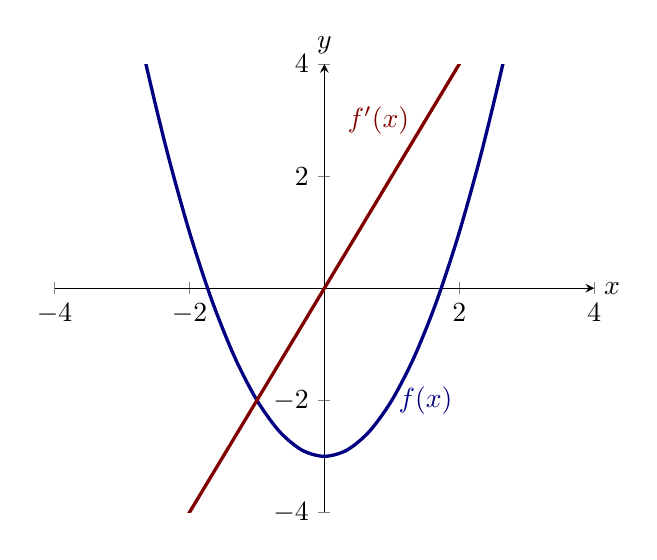
\begin{tikzpicture}
  \colorlet{background}{white}
  \colorlet{textColor}{black}
  \colorlet{penColor}{blue!50!black}
  \colorlet{penColor2}{red!50!black}
	\begin{axis}[
            domain=-4:4,
            xmax=4,
            xmin=-4,
            ymax=4,
            ymin=-4,
            axis lines =middle, xlabel=$x$, ylabel=$y$,
            every axis y label/.style={at=(current axis.above origin),anchor=south},
            every axis x label/.style={at=(current axis.right of origin),anchor=west}
          ]
          \addplot [very thick, penColor, smooth] {x^2-3};
          \addplot [very thick, penColor2, smooth] {2*x};
          \node at (axis cs:1.5,-2) {\color{penColor}$f(x)$};  
          \node at (axis cs:.8,3) {\color{penColor2}$f'(x)$};
        \end{axis}
\end{tikzpicture}
%\caption{A plot of $f(x) = x^3+1$ and $f'(x) = 3x^2$.}
%\label{figure:x^3+1}
\end{image}
\end{example}


Now we will consider a function that isn't defined on all of $\RR$.

\begin{example}
Compute 
\[
\ddx \sqrt{x+3}.
\]

Start by writing out the limit definition of the derivative where
$f(x) = \sqrt{x+3}$.
\begin{freeResponse}[given]
\[
\ddx f(x) = \lim_{h\to 0}\frac{\sqrt{(x+h)+3} - \sqrt{x+3}}{h}
\]
\end{freeResponse}
Now multiply by $\frac{\sqrt{(x+h)+3} + \sqrt{x+3}}{\sqrt{(x+h)+3} + \sqrt{x+3}}$.
\begin{freeResponse}[given]
\[
\ddx f(x) = \lim_{h\to 0}\frac{\left(\sqrt{(x+h)+3} - \sqrt{x+3}\right)\left(\sqrt{(x+h)+3} + \sqrt{x+3}\right)}{h\left(\sqrt{(x+h)+3} + \sqrt{x+3}\right)}
\]
\end{freeResponse}
Now expand the numerator.
\begin{freeResponse}[given]
\[
\ddx f(x) = \lim_{h\to 0}\frac{x+h+3 - (x+3)}{h\left(\sqrt{(x+h)+3} + \sqrt{x+3}\right)}
\]
\end{freeResponse}
Combine like-terms.
\begin{freeResponse}[given]
\[
\ddx f(x) = \lim_{h\to 0}\frac{h}{h\left(\sqrt{(x+h)+3} + \sqrt{x+3}\right)}
\]
\end{freeResponse}
Cancel $h$ from the numerator and denominator.
\begin{freeResponse}[given]
\[
\ddx f(x) = \lim_{h\to 0}\frac{1}{\sqrt{(x+h)+3} + \sqrt{x+3}}
\]
\end{freeResponse}
Take the limit as $h$ goes to $0$. 
\begin{freeResponse}[given]
\[
\ddx f(x) = \frac{1}{2\sqrt{x+3}}
\]
\end{freeResponse}
As a gesture of friendship, here is a plot of both $f(x)$ and $f'(x)$:
\begin{image}
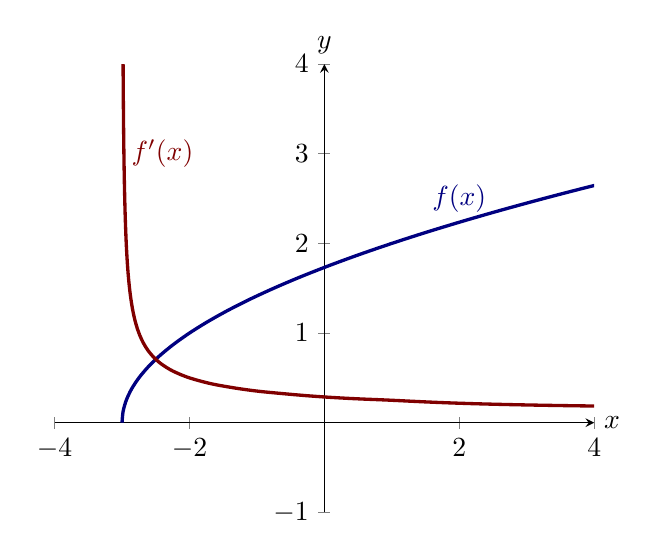
\begin{tikzpicture}
  \colorlet{background}{white}
  \colorlet{textColor}{black}
  \colorlet{penColor}{blue!50!black}
  \colorlet{penColor2}{red!50!black}
	\begin{axis}[
            domain=-4:4,
            xmax=4,
            xmin=-4,
            ymax=4,
            ymin=-1,
            axis lines =middle, xlabel=$x$, ylabel=$y$,
            every axis y label/.style={at=(current axis.above origin),anchor=south},
            every axis x label/.style={at=(current axis.right of origin),anchor=west}
          ]
          \addplot [very thick, penColor, smooth,domain=0:3] ({x^2-3},{x}); %% tricking out the plot
          \addplot [very thick, penColor2, smooth,samples=50,domain=.1:4] ({1/(4*x^2)-3},{x}); %% tricking out the plot
          \node at (axis cs:2,2.5) {\color{penColor}$f(x)$};  
          \node at (axis cs:-2.4,3) {\color{penColor2}$f'(x)$};
        \end{axis}
\end{tikzpicture}
\end{image}
\end{example}


Next we will consider the derivative a function that is not continuous
on $\RR$.


\begin{example}
Compute
\[
\ddx \frac{1}{3-x}.
\]

Start by writing out the limit definition of the derivative where
$f(x) = \frac{1}{3-x}$.
\begin{freeResponse}[given]
\[
\ddx f(x) = \lim_{h\to 0}\frac{\frac{1}{3-(x+h)} - \frac{1}{3-x}}{h}
\]
\end{freeResponse}
Now multiply by $\frac{(3-(x+h))(3-x)}{(3-(x+h))(3-x)}$.
\begin{freeResponse}[given]
\[
\ddx f(x) = \lim_{h\to 0}\frac{(3-x) - (3-(x+h))}{h(3-(x+h))(3-x)}
\]
\end{freeResponse}
Simplify the numerator
\begin{freeResponse}[given]
\[
\ddx f(x) = \lim_{h\to 0}\frac{h}{h(3-(x+h))(3-x)}
\]
\end{freeResponse}
Cancel $h$ from the numerator and denominator.
\begin{freeResponse}[given]
\[
\ddx f(x) = \lim_{h\to 0}\frac{1}{(3-(x+h))(3-x)}
\]
\end{freeResponse}
Take the limit as $h$ goes to $0$. 
\begin{freeResponse}[given]
\[
\ddx f(x) = \frac{1}{(3-x)^2}
\]
\end{freeResponse}
It is our pleasure to present a plot of both $f(x)$ and $f'(x)$:
\begin{image}
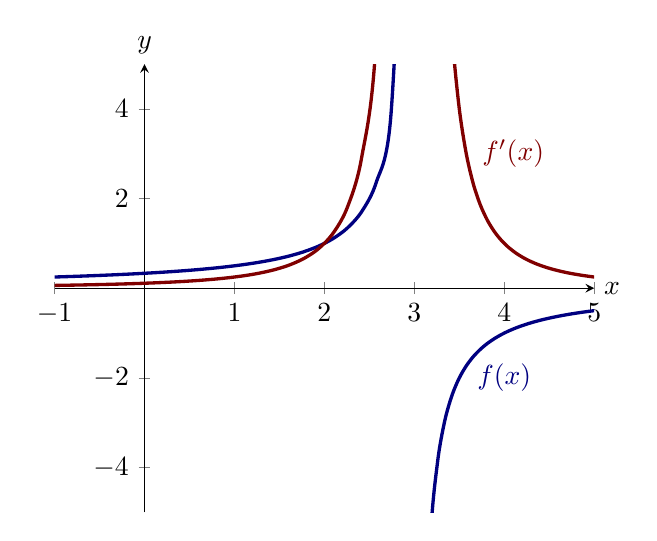
\begin{tikzpicture}
  \colorlet{background}{white}
  \colorlet{textColor}{black}
  \colorlet{penColor}{blue!50!black}
  \colorlet{penColor2}{red!50!black}
	\begin{axis}[
            xmax=5,
            xmin=-1,
            ymax=5,
            ymin=-5,
            %samples=100,
            axis lines =middle, xlabel=$x$, ylabel=$y$,
            every axis y label/.style={at=(current axis.above origin),anchor=south},
            every axis x label/.style={at=(current axis.right of origin),anchor=west}
          ]
          \addplot [very thick, penColor, smooth,domain=3.1:5] {1/(3-x)};
          \addplot [very thick, penColor, smooth,domain=-1:2.9] {1/(3-x)};
          \addplot [very thick, penColor2, smooth,domain=3.1:5] {1/(3-x)^2};
          \addplot [very thick, penColor2, smooth,domain=-1:2.9] {1/(3-x)^2};
          \node at (axis cs:4,-2) {\color{penColor}$f(x)$};  
          \node at (axis cs:4.1,3) {\color{penColor2}$f'(x)$};
        \end{axis}
\end{tikzpicture}
\end{image}
\end{example}


Recall that we started this discussion by thinking about the
\textit{MOOCulus-Mobile}.

\begin{example}
  If the position west of Columbus of the MOOCulus-Mobile is modeled by 
  \[
  s(t) = 36t^2 - 4.8t^3 \qquad \text{for $0\le t\le 5$,}
  \] 
  how do we find a formula for the velocity of the MOOCulus-Mobile?

  To solve this problem, we use the derivative. This is because the
  derivative computes the change in position with respect to time, and
  this is precisely the definition of velocity! Let's do this.

  Start by writing out the limit definition of the derivative where
  $s(t) = 36t^2 - 4.8t^3$.
  \begin{freeResponse}[given]
    \[
    \dd t s(t) = \lim_{h\to 0}\frac{36(t+h)^2 - 4.8(t+h)^3 - \left(36t^2 - 4.8t^3\right)}{h}
    \]
  \end{freeResponse}
  Now expand the numerator of the fraction.
  \begin{freeResponse}[given]
    \[
    \dd t s(t) = \lim_{h\to 0}\frac{36t^2 + 72th + 36h^2 - 4.8t^3 - 14.4t^2h - 14.4th^2 - 4.8h^3 - 36t^2 + 4.8t^3}{h}
    \]
  \end{freeResponse}
  Now combine like-terms.
  \begin{freeResponse}[given]
    \[
    \dd t s(t) = \lim_{h\to 0}\frac{72th + 36h^2 - 14.4t^2h - 14.4th^2 - 4.8h^3}{h}
    \]
  \end{freeResponse}
  Factor an $h$ from every term in the numerator.
  \begin{freeResponse}[given]
    \[
    \dd t s(t) = \lim_{h\to 0}\frac{h\left(72t + 36h - 14.4t^2 - 14.4th - 4.8h^2\right)}{h}
    \]
  \end{freeResponse}
  Cancel $h$ from the numerator and denominator.
  \begin{freeResponse}[given]
    \[
    \dd t s(t) = \lim_{h\to 0}\left(72t + 36h - 14.4t^2 - 14.4th - 4.8h^2\right)
    \]
  \end{freeResponse}
  Take the limit as $h$ goes to $0$. 
  \begin{freeResponse}[given]
    \[
    \dd t s(t) = 72t-14.4t^2
    \]
  \end{freeResponse}
  Behold the beauty of $s(t)$ and $s'(t)$:
  \begin{image}
    \begin{tikzpicture}
      \colorlet{background}{white}
      \colorlet{textColor}{black}
      \colorlet{penColor}{blue!50!black}
      \colorlet{penColor2}{red!50!black}
      \begin{groupplot}[group style={group size=2 by 1,horizontal sep=2cm}, width=0.5\textwidth]
        \nextgroupplot[
          clip=false,
          domain=0:5,
          xmax=5,
        xmin=0,
        ymax=300,
        ymin=0,
        axis lines =middle, 
        y label style={at={(axis description cs:-0.1,0.5)},rotate=90,anchor=south},
        x label style={at={(axis description cs:0.5,-.2)}},
        xlabel=hours into road-trip, ylabel=distance traveled in miles,
        ]
        \addplot [very thick, penColor, smooth] {36*x^2 - 4.8*x^3};
          \node at (axis cs:3,230) {\color{penColor}$s(t)$}; 
          \nextgroupplot[
            clip=false,
            domain=0:5,
            xmax=5,
            xmin=0,
            ymax=100,
            ymin=0,
            axis lines =middle, 
            y label style={at={(axis description cs:-0.1,0.5)},rotate=90,anchor=south},
            x label style={at={(axis description cs:0.5,-.2)}},
            xlabel=hours into road-trip, ylabel=velocity in miles per hour]
          \addplot [very thick, penColor2, smooth] {72*x-14.4*x^2};
          \node at (axis cs:3,95) {\color{penColor2}$s'(t)$};
      \end{groupplot}
    \end{tikzpicture}
  \end{image}
\end{example}








\end{document}
